% ******************************* Master Thesis Template **************************
% Please have a look at the README.txt file for info on how to use the template

\documentclass[a4paper,custommargin,times,numbered,printindex]{Classes/UCMScSeminar}
\usepackage{amsmath}
\usepackage{amssymb}
\usepackage{amsthm}
\usepackage{enumitem}
\usepackage{graphicx}
\usepackage{comment}
\usepackage{ragged2e}
\usepackage{hyperref}
\usepackage{booktabs}
\usepackage{xcolor,colortbl}
\definecolor{lavender}{rgb}{0.9, 0.9, 0.98}
%\usepackage{fancyhdr}
%\usepackage{acronym}
%\usepackage[default]{opensans}
%\usepackage{indentfirst}
%\setlength{\parindent}{1cm}
%\usepackage{setspace}
%\usepackage[avantgarde,nogrey]{quotchap}
\usepackage{xcolor}
%\usepackage[options]{subfigure}
%\usepackage[rightcaption]{sidecap}
%\usepackage{wrapfig}
\usepackage[portuguese]{babel}
\usepackage[utf8]{inputenc}


\newtheorem{teorema}{Teorema}%[chapter]
\newtheorem{definicao}{Definição}
\newtheorem{lema}[teorema]{Lema}
\newenvironment{demonstracao}{\paragraph{Demonstração}}{\hfill$\square$}
\newtheorem{corolario}[teorema]{Corolário}
\newtheorem{proposicao}[teorema]{Proposição}


% ******************************************************************************
% ******************************* Class Options ********************************
% *********************** See README for more details **************************
% ******************************************************************************
% *********************** RECOMMENDATIONS **************************************

% `a4paper'
%
% `11pt'´(default): Font Size 12pt is NOT recommended.

% ********************** SOME OPTIONS ******************************************
%
% `oneside' or `twoside'(default): Printing double side (twoside) or single
% side.
%
% `print': Use `print' for print version with appropriate margins and page
% layout. Leaving the options field blank will activate Online version.
%
% `langen`: This redefines the style to English language if the MSc Thesis is written in English.
%  The default language is Portuguese. In this case of using Portuguese there is no need to declare it.
%
% `index': For index at the end of the thesis
%
% `draft': For draft mode without loading any images (same as draft in book)
%
% `draftmode': Special draft mode with line numbers, images, and water mark with
% timestamp and custom text. Position of the text can also be modified.
%
% `abstract': To generate only the title page and abstract page with
% dissertation title and name.
%
% `chapter`: This option enables only the specified chapter and it's references
%  Useful for review and corrections.
%
% ************************* Custom Page Margins ********************************
%
% `custommargin`: Use `custommargin' in options to activate custom page margins,
% which can be defined in the preamble.tex. Custom margin will override
% print/online margin setup.
%
% *********************** Choosing the Fonts in Class Options ******************
%
% `times' : Times font with math support.
%
% `fourier': Utopia Font with Fourier Math font (Font has to be installed)
%            It's a free font.
%
% `customfont': Use `customfont' option in the document class and load the
% package in the preamble.tex
%
% default or leave empty: `Latin Modern' font will be loaded.
%
% ********************** Choosing the Bibliography style ***********************
%
% `authoryear': For author-year citation eg., Krishna (2013)
%
% `numbered': (Default Option) For numbered and sorted citation e.g., [1,5,2]
%
% `custombib': Define your own bibliography style in the `preamble.tex' file.
%              `\RequirePackage[square, sort, numbers, authoryear]{natbib}'.
%              This can be also used to load biblatex instead of natbib
%              (See Preamble)
%
% **************************** Choosing the Page Style *************************
%
% `default (leave empty)': For Page Numbers in Header (Left Even, Right Odd) and
% Chapter Name in Header (Right Even) and Section Name (Left Odd). Blank Footer.
%
% `PageStyleI': Chapter Name next & Page Number on Even Side (Left Even).
% Section Name & Page Number in Header on Odd Side (Right Odd). Footer is empty.
%
% `PageStyleII': Chapter Name on Even Side (Left Even) in Header. Section Number
% and Section Name in Header on Odd Side (Right Odd). Page numbering in footer


% ********************************** Preamble **********************************
% Preamble: Contains packages and user-defined commands and settings
% ******************************************************************************
% ****************************** Custom Margin *********************************

% Add `custommargin' in the document class options to use this section
% Set {innerside margin / outerside margin / topmargin / bottom margin}  and
% other page dimensions
\ifsetCustomMargin
  \RequirePackage[left=28mm,right=28mm,top=35mm,bottom=30mm]{geometry}
  \setFancyHdr % To apply fancy header after geometry package is loaded
\fi

% *****************************************************************************
% ******************* Fonts (like different typewriter fonts etc.)*************

% Add `customfont' in the document class option to use this section

\ifsetCustomFont
  % Set your custom font here and use `customfont' in options. Leave empty to
  % load computer modern font (default LaTeX font).
  \RequirePackage{helvet}
\fi

% *****************************************************************************
% ******************* COVER / CAPA ********************************************
\usepackage{pdfpages}

% *****************************************************************************
% **************************** Custom Packages ********************************

\usepackage[all]{xypic}
%\usepackage{algpseudocode}


% ********************Captions and Hyperreferencing / URL **********************

% Captions: This makes captions of figures use a boldfaced small font.
%\RequirePackage[small,bf]{caption}

\RequirePackage[labelsep=space,tableposition=top]{caption}
\renewcommand{\figurename}{Fig.} %to support older versions of captions.sty


% *************************** Graphics and figures *****************************

%\usepackage{rotating}
%\usepackage{wrapfig}

% Uncomment the following two lines to force Latex to place the figure.
% Use [H] when including graphics. Note 'H' instead of 'h'
%\usepackage{float}
%\restylefloat{figure}

% Subcaption package is also available in the sty folder you can use that by
% uncommenting the following line
% This is for people stuck with older versions of texlive
%\usepackage{sty/caption/subcaption}
\usepackage{subcaption}

% ********************************** Tables ************************************
\usepackage{booktabs} % For professional looking tables
\usepackage{multirow}

%\usepackage{multicol}
%\usepackage{longtable}
%\usepackage{tabularx}


% ***************************** Math ******************************

\usepackage{amsfonts}
\usepackage{amsmath}
\usepackage{amssymb}
\usepackage{stmaryrd} % \mapsfrom

%%%%%%%%%%
%%% Listagens
%%%%%%%%%%
\usepackage{listingsutf8}

\renewcommand{\lstlistingname}{Algoritmo}% Listing -> Algorithm
\renewcommand{\lstlistlistingname}{Lista de \lstlistingname s}% List of Listings -> List of Algorithms


 % definição da linguagem de programação
\lstset{language=C++,
  extendedchars=true,
  inputencoding=utf8,
  morekeywords={typedef,cin,cout,NULL,FILE},
  basicstyle=\small,
  frame=single
}

%  % definição da linguagem de programação
\lstdefinelanguage{algoritmo}{
  keywords={enquanto,para,se,entao,senao,fimse,fimpara,fimenquanto,faz,funcao,fimfuncao,return},
   extendedchars=true,
   inputencoding=utf8,
   morekeywords={faz,funcao,return},
   basicstyle=\small,
   frame=single
}

% para lidar com o UTF8
\lstset{literate=
  {á}{{\'a}}1 {é}{{\'e}}1 {í}{{\'i}}1 {ó}{{\'o}}1 {ú}{{\'u}}1
  {Á}{{\'A}}1 {É}{{\'E}}1 {Í}{{\'I}}1 {Ó}{{\'O}}1 {Ú}{{\'U}}1
  {à}{{\`a}}1 {è}{{\`e}}1 {ì}{{\`i}}1 {ò}{{\`o}}1 {ù}{{\`u}}1
  {À}{{\`A}}1 {È}{{\'E}}1 {Ì}{{\`I}}1 {Ò}{{\`O}}1 {Ù}{{\`U}}1
  {ä}{{\"a}}1 {ë}{{\"e}}1 {ï}{{\"i}}1 {ö}{{\"o}}1 {ü}{{\"u}}1
  {Ä}{{\"A}}1 {Ë}{{\"E}}1 {Ï}{{\"I}}1 {Ö}{{\"O}}1 {Ü}{{\"U}}1
  {â}{{\^a}}1 {ê}{{\^e}}1 {î}{{\^i}}1 {ô}{{\^o}}1 {û}{{\^u}}1
  {Â}{{\^A}}1 {Ê}{{\^E}}1 {Î}{{\^I}}1 {Ô}{{\^O}}1 {Û}{{\^U}}1
  {Ã}{{\~A}}1 {ã}{{\~a}}1 {Õ}{{\~O}}1 {õ}{{\~o}}1 {ñ}{{\~n}}1
  {œ}{{\oe}}1 {Œ}{{\OE}}1 {æ}{{\ae}}1 {Æ}{{\AE}}1 {ß}{{\ss}}1
  {ű}{{\H{u}}}1 {Ű}{{\H{U}}}1 {ő}{{\H{o}}}1 {Ő}{{\H{O}}}1
  {ç}{{\c c}}1 {Ç}{{\c C}}1 {«}{{\guillemotleft}}1 {»}{{\guillemotright}}1
  {€}{{\EUR}}1 {£}{{\pounds}}1
}


% ******************************* Line Spacing *********************************

% Choose linespacing as appropriate. Default is one-half line spacing

% \doublespacing
% \onehalfspacing
% \singlespacing


% ************************ Formatting / Footnote *******************************

% Don't break enumeration (etc.) across pages in an ugly manner (default 10000)
%\clubpenalty=500
%\widowpenalty=500

%\usepackage[perpage]{footmisc} %Range of footnote options


% *****************************************************************************
% *************************** Bibliography  and References ********************

%\usepackage{cleveref} %Referencing without need to explicitly state fig /table

% Add `custombib' in the document class option to use this section
\ifuseCustomBib
   \RequirePackage[square, sort, numbers, authoryear]{natbib} % CustomBib

% If you would like to use biblatex for your reference management, as opposed to the default `natbibpackage` pass the option `custombib` in the document class. Comment out the previous line to make sure you don't load the natbib package. Uncomment the following lines and specify the location of references.bib file

%\RequirePackage[backend=biber, style=numeric-comp, citestyle=numeric, sorting=nty, natbib=true]{biblatex}
%\bibliography{References/references} %Location of references.bib only for biblatex

\fi

% changes the default name `Bibliography` -> `References'
\ifisLangPt
  \renewcommand{\bibname}{Bibliografia}
\else
  \renewcommand{\bibname}{References}
\fi


% *****************************************************************************
% *************** Changing the Visual Style of Chapter Headings ***************

% Uncomment the section below. Requires titlesec package.

%\RequirePackage{titlesec}
%\newcommand{\PreContentTitleFormat}{\titleformat{\chapter}[display]{\scshape\Large}
%{\Large\filleft{\chaptertitlename} \Huge\thechapter}
%{1ex}{}
%[\vspace{1ex}\titlerule]}
%\newcommand{\ContentTitleFormat}{\titleformat{\chapter}[display]{\scshape\huge}
%{\Large\filleft{\chaptertitlename} \Huge\thechapter}{1ex}
%{\titlerule\vspace{1ex}\filright}
%[\vspace{1ex}\titlerule]}
%\newcommand{\PostContentTitleFormat}{\PreContentTitleFormat}
%\PreContentTitleFormat


% ******************************************************************************
% ************************* User Defined Commands ******************************
% ******************************************************************************

% *********** To change the name of Table of Contents / LOF and LOT ************

%\renewcommand{\contentsname}{My Table of Contents}
%\renewcommand{\listfigurename}{My List of Figures}
%\renewcommand{\listtablename}{My List of Tables}


% ********************** TOC depth and numbering depth *************************

\setcounter{secnumdepth}{2}
\setcounter{tocdepth}{2}


% ******************************* Nomenclature *********************************

% To change the name of the Nomenclature section, uncomment the following line

%\renewcommand{\nomname}{List of Symbols}


% ********************************* Appendix ***********************************

% The default value of both \appendixtocname and \appendixpagename is `Appendices'. These names can all be changed via:

%\renewcommand{\appendixtocname}{List of appendices}
%\renewcommand{\appendixname}{Appndx}
\ifisLangPt
  \renewcommand{\appendixname}{Anexo}
%  \renewcommand{\appendixtocname}{Lista de Ap\textasciicircum endices}
\fi

% ******************************** Draft Mode **********************************

% Uncomment to disable figures in `draftmode'
%\setkeys{Gin}{draft=true}  % set draft to false to enable figures in `draft'

% These options are active only during the draft mode
% Default text is "Draft"
%\SetDraftText{DRAFT}

% Default Watermark location is top. Location (top/bottom)
%\SetDraftWMPosition{bottom}

% Draft Version - default is v1.0
%\SetDraftVersion{v1.1}

% Draft Text grayscale value (should be between 0-black and 1-white)
% Default value is 0.75
%\SetDraftGrayScale{0.8}


%% Todo notes functionality
%% Uncomment the following lines to have todonotes.

%\ifsetDraft
%	\usepackage[colorinlistoftodos]{todonotes}
%	\newcommand{\mynote}[1]{\todo[author=kks32,size=\small,inline,color=green!40]{#1}}
%\else
%	\newcommand{\mynote}[1]{}
%	\newcommand{\listoftodos}{}
%\fi

% Example todo: \mynote{Hey! I have a note}




% ************************ Thesis Information & Meta-data **********************
% Thesis title and author information, reference file for biblatex

% ************************ Thesis Information **********************
%% The title of the thesis
\title{Criptografia RSA}

%% The full name of the author
\author{José Diogo Songo}

%% Logo
\crest{
\includegraphics[width=0.4\textwidth]{UC_fundoclaro.png}}

%% Uncomment the appropriate lines
\spareaLangEn{Applied Analysis and Computation}
%\spareaLangEn{Statistics, Optimization and Mathematics in Finance}
%\spareaLangEn{Pure Mathematics}
\spareaLangPt{An\'{a}lise Aplicada e Computa\c{c}\~{a}o}
%\spareaLangPt{Estat\'{\i}stica, Otimiza\c{c}\~{a}o e Matem\'{a}tica Financeira}
%\spareaLangPt{Matem\'{a}tica Pura}

%% Full title of the Program
\ifisLangEn
  \degree{Research Seminar \\[2mm] Seminário de Investigação}
\else
  \degree{Seminário de Investigação \\[2mm] Research Seminar}
\fi


%% Submission date
% Default is set as {\monthname[\the\month]\space\the\year}
%%
%% Uncomment the appropriate line and update with the actual defense date in the given format
%%
%\degreedate{September 2016}
%\degreedate{Janeiro 2019 / January 2019}
\ifisLangEn
  \degreedate{January 2024 / Janeiro 2024}
\else
  \degreedate{Janeiro 2024 / January 2024}
\fi


% ***************************** Abstract Separate ******************************
% To printout only the titlepage and the abstract with the MSc title and the
% author name for submission to the Registry, use the `abstract' option in
% the document class.

\ifdefineAbstract
 \pagestyle{empty}
 \includeonly{Abstract/abstract}
\fi

% ***************************** Chapter Mode ***********************************
% The chapter mode allows user to only print particular chapters with references
% Title, Contents, Frontmatter are disabled by default
% Useful option to review a particular chapter or to send it to supervisor.
% To use choose `chapter' option in the document class

\ifdefineChapter
 \includeonly{Chapter3/chapter3}
\fi

% ******************************** Front Matter ********************************
\begin{document}

% COVER UC
% The cover should be prepared in the University template (file 'Capa_Dissertacao_TPL-A4.docx') and saved as a pdf file to include here
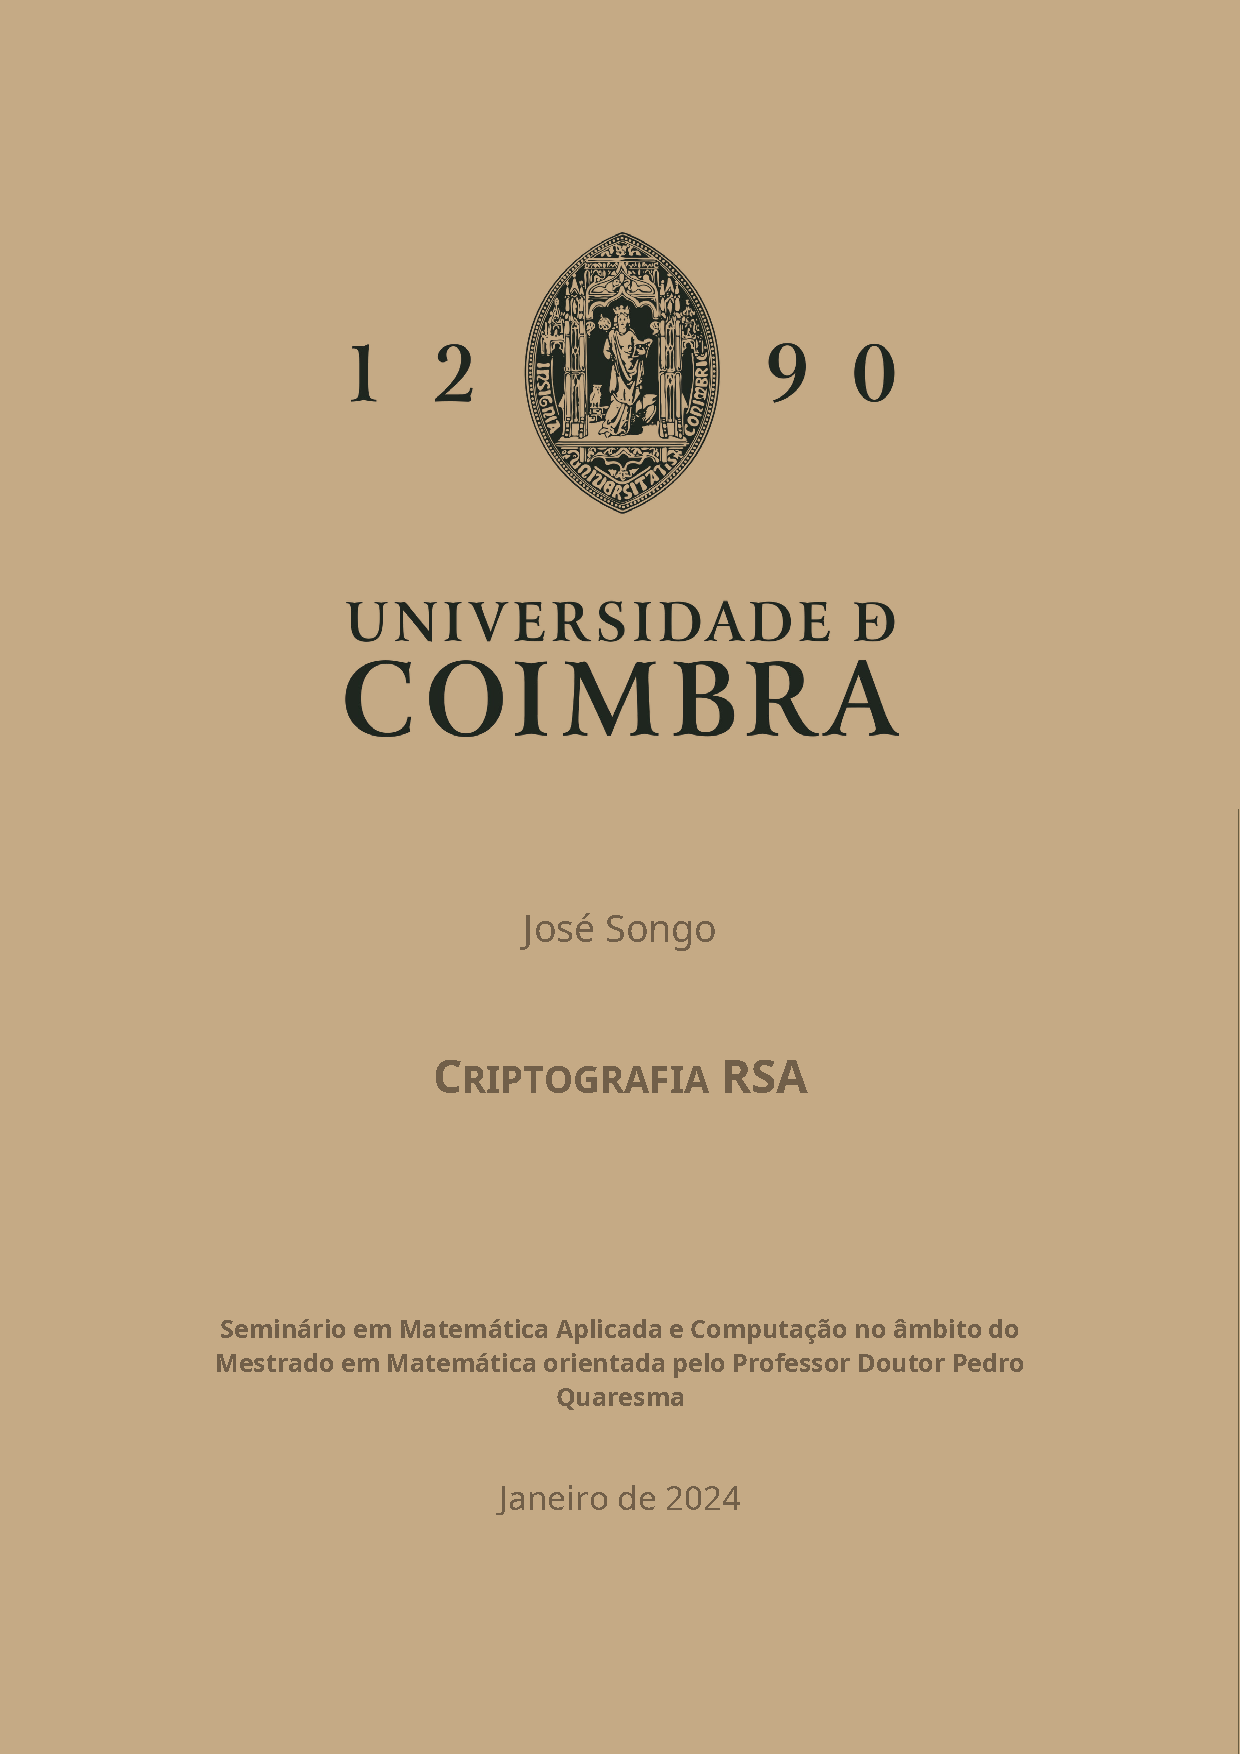
\includepdf{Cover/Capa_Dissertacao_TPL-A4.pdf}


\frontmatter

\begin{titlepage}
  \vspace*{30mm}
  \maketitle
\end{titlepage}


% ************************** Thesis Acknowledgements *****************************

\begin{acknowledgements}


Agradeço ao professor Pedro Quaresma, que aceitou orientar o meu projeto, revelando uma especial atenção às minhas ideias. Os seus conselhos e sugestões bem como a valorização do trabalho desenvolvido foram determinantes para alcançar este resultado.


\end{acknowledgements}

% ************************** Thesis Abstract *****************************
% Use `abstract' as an option in the document class to print only the titlepage and the abstract.
\begin{abstract}
\ifisLangEn

If the Dissertation is in Portuguese, do not write here anything.
This is where you write your abstract in English.

% ************************************************************************
%
% As linhas seguintes definem o `resumo' em portugu\^{e}s apenas no caso
% da l\'{\i}ngua utilizada ser o ingl\^{e}s. Caso contr\'{a}rio, ser\~{a}o ignoradas.
%
% ************************************************************************

  \cleardoublepage
  \setsinglecolumn
  \chapter*{\centering \Large Resumo}
  \thispagestyle{empty}

\else
  %Aqui escreve o Resumo em Portugu\^{e}s no caso da disserta\c{c}\~{a}o usar o Ingl\^{e}s.

    A criptografia RSA revolucionou a segurança digital com o seu procedimento de chaves pública e privada, em contraponto com as cifras de chaves simétricas cuja gestão das chaves é muito difícil de gerir em ambientes com muitos intervenientes. A criptoanálise, por sua vez, desempenha um papel fundamental na avaliação e no aprimoramento da segurança dos sistemas criptográficos, buscando constantemente formas de tornar as comunicações digitais mais seguras e protegidas contra ameaças cibernéticas.

    Neste texto apresentam-se as implementações dos diferentes métodos descritos no trabalho de seminário, nomeadamente, os algoritmos para os métodos de deslocamento simples, linear e RSA.
    
    No final, foi feito um estudo comparativo dos métodos acima mencionados.
\fi
\end{abstract}


% *********************** Adding TOC and List of Figures ***********************

\tableofcontents

%\listoffigures

%\listoftables

% *********************** Index of Nomenclature (Optional) ***********************
%
%% printnomencl should be commented out, if you are using a list of Nomenclature
%
% ********************************************************************************

%% In case you don’t like the name of the nomenclature, just redefine the \nomname macro, e. g.
%\renewcommand{\nomname}{List of symbols}

%\printnomencl

%% It uses the package nomencl
%%\printnomencl[space] space can be set as 2em between symbol and description
%%\printnomencl[3em]

%%%% IMPORTANT: The nomencl package only creates a fyle thesis.nlo.
%%%%            You need to create the file thesis.nls that contains your nomenclature list properly ordered.
%%
%% In order to do that and to include the list in the pdf the compile sequence must be:
%% run pdfLaTeX
%% run makeindex thesis.nlo -s nomencl.ist -o thesis.nls
%% then rerun pdfLaTeX


% ******************************** Main Matter *********************************
\mainmatter

%*******************************************************************************
%*********************************** First Chapter *****************************
%*******************************************************************************


\chapter{Introdução}


A criptografia é uma técnica antiga e importante utilizada para proteger informações confidenciais por meio da codificação e descodificação de mensagens. Ela desempenha um papel essencial na segurança da comunicação, impossibilitando que terceiros não autorizados compreendam ou acessem o conteúdo das mensagens.~\cite{Quaresma2008a,Quaresma2009a}.

Um dos exemplos mais simples de criptografia é a cifra de Júlio César, também conhecida como cifra de deslocamento ou cifra de substituição. Essa técnica foi usada pelo renomado imperador romano Júlio César (100aC -- 44aC) para enviar mensagens secretas durante as suas ações militares.

A cifra de Júlio César funciona substituindo cada letra do alfabeto por outra, deslocando um número fixo de posições para a esquerda ou direita no alfabeto. Por exemplo, se usarmos um deslocamento de 3 posições para a direita, a letra ``a'' seria substituída pela letra ``d'', ''b'' seria substituída por ``e'', e assim por diante. Ao chegar ao fim do alfabeto, volta-se ao início, por exemplo ``x'' passa a ``a'',``y'' passa a ``b'' e ``z'' passa a ``c''.

Essa técnica simples demonstra os princípios fundamentais da criptografia, onde a informação original é escondida de uma maneira específica para ocultar seu significado, e somente aqueles que possuem a chave podem decifrar a mensagem.

No entanto, a cifra de Júlio César é bastante vulnerável a ataques de força bruta, pois há um número limitado de combinações possíveis. Por isso, ela é considerada uma forma trivial de criptografia e não é adequada para proteger informações sensíveis nos dias atuais. Hoje em dia, algoritmos mais complexos e seguros são utilizados para garantir a segurança das comunicações, como AES (Advanced Encryption Standard) e RSA (Rivest-Shamir-Adleman), oferecendo níveis avançados de proteção.
%*******************************************************************************
%****************************** Second Chapter *********************************
%*******************************************************************************



\chapter{Fundamentos Matemáticos}
\label{sec:FundamentosMatematicos}

Em seguida são apresentados fundamentos teóricos matemáticos indispensáveis ao estudo da criptografia.

\section{Funções Unidirecionais}

\begin{definicao}[Função Unidirecional]
\label{def:funcaoUnidirecional}
Uma função $f$ de um conjunto $X$ para um conjunto $Y$ é dita uma função unidirecional («one-way function») se $f(x)$ é «fácil de calcular» para todo o $x \in X$, mas «essencialmente para todos» os elementos $y \in Im(f)$ é «computacionalmente difícil» achar um $x \in X$ tal que $f(x)=y.$
\end{definicao}

\begin{definicao}[Função Unidirecional com Escapatória]
\label{def:funcaoUnidirecionalEscapatoria}
Uma função unidirecional com escapatória é uma função unidirecional $f: X \longrightarrow Y$ com a propriedade de que dado algum tipo de informação adicional torna-se possível encontrar, para um dado $y \in Im(f)$ e um dado $x \in X$ tal que $f(x)=y$.
\end{definicao}



%PEDIR AO PROFESSOR PARA VERIFICAR ESSA DEFINIÇÃO

\section{Resultados da Teoria dos Números}

\begin{definicao}[Divisibilidade]: 
\label{def:divisibilidade}
Dados $a,b \in \mathbb{Z}$, com $a\neq0$, diz-se que, $a$ divide $b$, e escreve-se $a|b$, se existe $q \in \mathbb{Z}$ tal que $b=aq$.
\end{definicao}

Convenção: Quando se escreve $a|b$ está implícito que a $a \neq 0$.

Se $a|b$ também se diz que $a$ é um divisor de b, que b é um múltiplo de $a$ ou que $b$ é divisível por $a$.

Se $a$ não divide $b$, escreve-se $a \nmid b$.

Para quaisquer $a,b,c \in \mathbb{Z}$ tem-se:

\begin{enumerate}
    \item{ $a|0, 1|a \;e\;a|a$};
    \item{ $a|b 	\Leftrightarrow a|-b \Leftrightarrow -a|b$};
    \item{$a|b \land b|c \Leftrightarrow a|c$};
    \item Para quaisquer $x,y \in \mathbb{Z}, a|b \land a|c \Leftrightarrow a|bx + cy$;
    \item $a|1 \Leftrightarrow a=\pm b$;
    \item $a,b \in \mathbb{N} \land a|b \Leftrightarrow a \leq b$;
    \item Um inteiro não nulo tem um número finito de divisores.
\end{enumerate}


\begin{teorema}[Algoritmo da Divisão Inteira] 
\label{teo:AlgoritmoDivisaoInteira}
Dados $a,b \in \mathbb{Z}$, com $a \neq 0$, existem $q,r \in \mathbb{Z}$, únicos, tais que $$b=aq, \; com \; 0\leq r < |a|$$
$q$ e $r$ são, respetivamente, o quociente e o resto da divisão inteira de $b$ por $a$.
\end{teorema}

Observações:

\begin{enumerate}
    \item $a|b$ se e só se o resto da divisão inteira de $b$ por $a$ é zero.
    \item Em $C/C++$, os operadores ``$/$'' e ``\%'' dão-nos o quociente e o resto da divisão inteira (desde que o divisor e o dividendo sejam inteiros).
\end{enumerate}

\begin{definicao}[Congruência $\mod m$]
\label{def:congruenciamodm}
Para $m \in \mathbb{N}$ a relação de congruência módulo $m$ é a relação definida em $\mathbb{Z}$ por $$a \equiv b (mod\;m) \Leftrightarrow  m|a-b, \; a,b \in \mathbb{Z}$$
Se $a \equiv b (\mod m)$ diz-se que $a$ é congruente módulo $m$ com $b$.
\end{definicao} 

Observe-se que $a \equiv b (mod\;m)$ se e só se $a$ e $b$ têm o mesmo resto quando dividos por $m$.

Propriedades da congruência

\begin{enumerate}
    \item $a \equiv a\;(mod\;m)$ (Reflexividade)
    \item $a \equiv b\;(mod\;m)\Rightarrow b\equiv a\;(mod\; m)$
    \item $a \equiv b\;(mod\;m) \land a \equiv b\;(mod\; m) \Rightarrow a\;\equiv c(mod\; m)$
    \item $a \equiv b\;(mod\;m) \land c \equiv d(mod\;m) \Rightarrow a + c \equiv b+d \;(mod\;m)$
    \item $a \equiv b\;(mod\; m) \land c \equiv d(mod\; m) \Rightarrow ac \equiv bd\;(mod\; m)$
    \item $a \equiv b\;(mod\; m)\Rightarrow mdc(a.m)=mdc\;(b,m)$
    \item $ab \equiv ac\;(mod\; m)\Rightarrow b \equiv c\;(mod \frac{m}{mdc\;(a,m)})$
\end{enumerate} 
Das propriedades 1, 2 e 3 resulta que, para $m \in \mathbb{N}$, a relação de congruência módulo $m$ é uma relação de equivalência em $\mathbb{Z}$.

As classes de equivalência desta relação de equivalência chamam-se classes de congruência módulo m.

A classe de congruência módulo $m$ a que pertence $a\in \mathbb{Z}$ é representada por $[a]_m$ ou $\overline{a}$.

Uma vez que $a \in \mathbb{Z}$ é congruente módulo $m$ com o resto da divisão inteira por $m$, e os $m$ restos possíveis são $0,1,2,\dotsc,m-2$ e $m-1$ classes, conclui-se que há $m$ classes de congruência módulo $m$:
$[0]_m,[1]_m,\dotsc,[m-1]_m$

Para $m \in \mathbb{N}$, por $\mathbf{Z}_m$ representa-se o conjunto das classes de congruência módulo $m$, isto é, $$\mathbb{Z}_m={[0]_m,[1]_m,\dotsc,[m-1]_m}$$
Uma vez que $$a \equiv c(mod\; m) \land b \equiv d(mod\; m) \Rightarrow a + b \equiv c + d(mod\; m)$$
pode definir-se uma operação em $\mathbb{Z}_m$(adição de classes de congruência) por $[a]_m + [a]_m =[a +b]_m$
$$(\mathbb{Z}_m,+) \; é \; um \; grupo \;abeliano$$
Neste grupo o elemento neutro é $[0]_m$ e o simétrico de $[a]_m$ é $[-a]_m=[m-a]_m$\\

\begin{definicao}[Máximo Divisor Comum] Sejam $a,b \in \mathbb{Z}$ com $a \neq 0$ ou $b \neq 0$ e considere-se $D=\{c \in \mathbb{Z}: c|a \land c|b\}$.
\end{definicao}

$D \neq \emptyset$, porque $1 \in D$ e $D$ é finito porque um inteiro não nulo tem um número finito de divisores.

Então $D$ tem um máximo ao qual se chama máximo divisor comum de $a$ e $b$. Esse máximo é representado por $mdc(a,b)$.

Se $mdc(a,b)=1$ diz-se que os inteiros $a$ e $b$ são primos entre si ou que $a$ é primo com $b$.

Propriedades dos máximos divisores comum

Para quaisquer $a,b,c \in \mathbb{Z} \backslash \{0\}$, tem-se:
\begin{enumerate}
    \item $mdc(a,b)=mdc(b,a)=mdc(a,-b);$
    \item $mdc \left(\frac{a}{mdc(a,b)},\frac{b}{mdc(a,b)}\right)=1$
    \item $mdc(a,b)$ é o menor elemento positivo de $\{ax + by:\;x,y \in \mathbb{Z}\}$
    \item Se $x,y \in \mathbb{Z}$ são tais que $mdc(a.b)=ax + by$ então $mdc(x,y)=1$;
    \item $mdc(a,b)$ é o único divisor comum, positivo, de $a$ e $b$ tal que:
    $$x \in \mathbb{Z}\backslash \{0\} \land x|a \land x|b \Rightarrow x|mdc(a.b)$$
    \item $a|bc \land mdc(a,b)=1 \Rightarrow a|c$
\end{enumerate}
Para calcular o máximo divisor comum de $a,b \in \mathbb{Z}\backslash\{0\}$ usa-se o algoritmo de Euclides.

\begin{teorema}[Algoritmo de Euclides] 
\label{teo:AlgoritmoEuclides}
Sejam $a \in \mathbb{N}$ e $b \in \mathbb{Z}$. Aplicando sucessivamente o algoritmo da divisão obtém-se: 

\begin{align*}
    & b=aq_1 + r_1,\;0 < r_1 < a\\
    & a=r_1q_2 + r_2,\;0 < r_2 < r_1\\
    &r_1=r_2q_3 + r_3, \;0 < r_3 < r_2\\
                \vdots\\
    &r_{k-2}=r_{k-1}q_k + r_k, \;0 < r_k < r_{k-1}\\
    &r_{k-1}=r_kq_{k+1}
\end{align*}
para um dado $k \in \mathbb{N}\;(r_0:=a\;e\;r_{-1}:=b)$

Então $mdc(a,b)=r_k$.
\end{teorema}

\begin{proposicao}[Congruências Lineares]
Sejam $m \in \mathbb{N},\; a,b \in \mathbb{Z}$ com $mdc(a,m)=1$. A congruência $ax \equiv b(mod\;m)$ tem solução e o conjunto das soluções é uma classe de congruência módulo $m$.
\end{proposicao}

Método de resolução de $ax \equiv b(mod\;m)$ com $mdc(a,m)=1$:

Usando o algoritmo de Euclides determinam-se $x_0,y_0 \in \mathbb{Z}$ tais que $ax_0+my_0=1$. De $ax_0\equiv1(mod\;m)$ resulta que $ax_0\equiv b(mod\;m)$.

O conjunto das soluções de $ax\equiv b(mod\;m)$ é $[x_0b]_m$.

\begin{proposicao}[Congruências Lineares---Caso geral] Sejam $m \in \mathbb{N},a,b\in\mathbb{Z}$ e $d=mdc(a,m)$. A congruência $ax\equiv b(mod m)$ tem solução se e só se $d|b$.
\end{proposicao}

Se $d|b$ então $$ax\equiv b(mod \; m) \Leftrightarrow \frac{a}{d}x\equiv\frac{b}{d}\left(mod\frac{m}{d}\right)$$
e o conjunto das soluções é a união de d classes de congruência módulo m.\\

\begin{proposicao}[Inverso Multiplicativo]: Se $mdc(a,m)=1$, então $[a]_m$ é invertível em $\mathbb{Z}_m$ e , sendo $x_0,y_0 \in \mathbb{Z}$ tais que $ax_0+my_0=1$, tem-se que:$$[a]_m^{-1}=[x_0]_m$$
\end{proposicao}

Notar que se $mdc(a,m) > 1, [a]_m$ não é invertível\\
Os elementos invertíveis em $(\mathbb{Z}_m,.)$ são os elementos de $\{[a]_m:mdc(a,m)=1\}$.\\
Observação: $(\mathbb{Z}_m\backslash \{[0]_m\},.)$ é um grupo, se e só se $m$ é primo.\\

\begin{teorema}[Grupo multiplicativo]Seja $U_m=\{[a]_m:mdc(a,m)=1\}$. Consideremos $m \in \mathbb{N}$. $U_m$ é um grupo para a multiplicação de classes de congruência módulo $m$.
\end{teorema}

Notações:
\begin{enumerate}
    \item Quando se trabalha em $\mathbb{Z}_m$ muitas vezes representa-se $[a]_m$ apenas por $r$, sendo \mbox{$r \in \{0,1,\ldots,m-1\}$} o resto da divisão inteira por $a$ por $m$;
    \item Sendo $a \in \mathbb{Z}$ e $m \in \mathbb{N}$, é usual representar por $amod\;m$ o resto da divisão inteira de $a$ por $m$;
    \item Se $mdc(a,m)=1$, por $a^{-1} \mod\;m$ representa-se o inverso de $[a]_m$ em $\mathbb{Z}_m$
\end{enumerate}

\begin{definicao}[Menor Múltiplo Comum] Dados $a,b \in \mathbb{Z}\backslash \{0\}$, um inteiro não nulo $c$ é um múltiplo comum de $a$ e $b$ se $a|c$ e $b|c$.
\end{definicao}

Sejam $a,b \in \mathbb{Z}\backslash \{0\}$ e considere-se $M=\{c \in \mathbb{N}:a|c \land b|c\}$.\\

$M \neq \emptyset$ porque $|ab| \in M$. Além disso, $M \subseteq \mathbb{N}$. Então $M$ tem um mínimo ao qual se chama menor múltiplo comum de $a$ e $b$.\\
Esse mínimo é representado por $mmc(a,b).$\\

Para quaisquer $a,b \in \mathbb{Z} \backslash \{0\}$, tem-se:
\begin{enumerate}
    \item $mmc(a,b)$ é o único múltiplo comum, positivo, de $a$ e $b$ tal que:$$x \in \mathbb{Z} \land a|x \land b|x \Rightarrow mmc(a,b)|x$$
    \item Se $n \in \mathbb{N}$ é um divisor comum de $a$ e $b$ então
    $$mmc\left(\frac{a}{n},\frac{b}{n}\right)$$
    \item $mmc(a,b)mdc(a,b)=|ab|$
\end{enumerate}
O menor múltiplo comum de $a,b \in \mathbb{Z} \backslash \{0\}$ pode ser calculado usando o algoritmo de Euclides e a propriedade 3.\\

\begin{definicao}[máximo divisor comum---caso geral] 
$n \in \mathbb{N},n \ge 2,a_1,a_2,\dotsc,a_n \in \mathbb{Z}$ não todos nulos. O máximo divisor comum de $a_1,a_2,\dotsc,a_n$ é o menor dos divisores comuns positivos de $a_1,a_2,...,a_n$. Representa-se por $mdc(a_1,a_2,\dotsc,a_n)$


Propriedades:
\begin{enumerate}
    \item $mdc(a_1,a_2,\dotsc,a_n)$ é o menor inteiro positivo da forma\\$a_1x_1+a_2x_2+\dotsc+a_nx_n$, com $x_1,x_2,\dotsc,x_n \in \mathbb{Z}$
    \item $mdc(a_1,a_2,\dotsc,a_n)$ é o único divisor comum positivo, de $a_1,a_2,\dotsc,a_n$ que é múltiplo de qualquer divisor comum de $a_1,a_2,\dotsc,a_n$
    \item $mdc(a_1,a_2,\dotsc,a_n)=mdc(mdc(a_1,a_2,\dotsc,a_{n-1}),a_n)$
\end{enumerate}
\end{definicao}

\begin{definicao}
Os inteiros $a_1,a_2,\dotsc,a_n$ são primos dois a dois se $mdc(a_i,a_j)=1$, para $i,j=1,2,\dotsc,n$, com $i \neq j$.
$$a_1,a_2,\dotsc,a_n \text{ são primos dois a dois}$$
$$\downarrow $$
$$a_1,a_2,\dotsc,a_n \text{ são primos entre si}$$
Notar que a implicação reciproca é falsa.
\end{definicao}

\begin{definicao}: $n \in \mathbb{N},n \ge 2,a_1,a_2,\dotsc,a_n \in \mathbb{Z}$ não todos nulos. O menor múltiplo comum de $a_1,a_2,\dotsc,a_n$ é o menor dos múltiplos comuns positivos de $a_1,a_2,\dotsc,a_n$. Representa-se por \linebreak $mmc(a_1,a_2,\dotsc,a_n)$.\\

Propriedades:
\begin{enumerate}
    \item $mmc(a_1,a_2,\dotsc,a_n)$ é o único múltiplo comum, positivo, de $a_1,a_2,\dotsc,a_n$ que divide qualquer múltiplo comum de $a_1,a_2,\dotsc,a_n$;
    \item $mmc(a_1,a_2,\dotsc,a_n)=mmc(mmc(a_1,a_2,\dotsc,a_{n-1}),a_n)$
\end{enumerate}
Para $n \leq 3$, em geral,\\$mmc(a_1,a_2,\dotsc,a_n)=mmc(mmc((a_1,a_2,\dotsc,a_{n-1}),a_n) \neq |a_1,a_2,\dotsc,a_n|$
\end{definicao}

\begin{definicao} Um inteiro $p>1$ diz-se um número primo se os únicos divisores positivos de $p$ são 1 e $p$.
Um inteiro diz-se composto se não é primo.
\end{definicao}

\begin{teorema} $p$ número primo; $a_1,a_2,\dotsc,a_n \in \mathbb{Z}$ $$p|a_1a_2\dots ca_n\;\Rightarrow \;p|a_1 \lor p|a_2\lor \dots c \lor p|a_n$$
\end{teorema}

\begin{teorema}[Teorema Fundamental da Aritmética] Todo o inteiro maior que $1$ pode ser escrito, de modo único(a menos da ordem dos fatores), como produto de números primos.
\end{teorema}

\begin{teorema}[Fatorização de Números Primos] Se $a=p_1^{\alpha_1}p_2^{\alpha_2}\dotsc p_k^{\alpha_k}$ e $a=p_1^{\beta_1}p_2^{\beta_2}\dotsc p_k^{\beta_k}$ onde $p_1,\dotsc p_k$ são números primos dois a dois e $\alpha_1,\dotsc,\alpha_k$,$\beta_1,\dotsc,\beta_k \in \mathbb{N}_0$, então  $$a|b \Leftrightarrow(\alpha_i \leq \beta_i,i=1,\dotsc,k)$$
$$mdc(a,b)=p_1^{min\{\alpha_1,\beta1\}}p_2^{min\{\alpha_2,\beta2\}}\dotsc p_k^{min\{\alpha_k,\beta_k\}}$$
e
$$mdc(a,b)=p_1^{max\{\alpha_1,\beta1\}}p_2^{max\{\alpha_2,\beta2\}}\dotsc p_k^{max\{\alpha_k,\beta_k\}}$$
\end{teorema}

\begin{definicao}[Função de Euler]: a função de Euler é a função $\phi : \mathbb{N} \Rightarrow \mathbb{N}$ definida por:$$\phi ( n)=|{a \in \mathbb{N}:a \leq n\;e \;mdc(a,n)=1}|,\;n\in \mathbb{N}$$
\end{definicao}

\begin{teorema}
\label{teo:teoremaA}
 A função $\phi$ é multiplicativa, isto é, se $m,n \in \mathbb{N}$ são tais que $mdc(m,n)=1$, então $$\phi(mn)=\phi(m) \phi(n)$$
 \end{teorema}
 
\begin{teorema}    
 Sejam, $p_1,p_2,\dotsc ,p_n$ números primos distintos dois a dois e\\ $\alpha_1,\alpha_2,\dotsc,\alpha_n \in \mathbb{N}$
$$\phi(p_1^{\alpha_1} \dotsc p_k^{\alpha_k} )=(p_1^{\alpha_1} -p_1^{\alpha-1} )\dotsc (p_k^{\alpha_k} -p_k^{\alpha-1} )$$
\end{teorema}
\begin{teorema}[Pequeno Teorema de Fermat]
\label{teo:PequenoTeoremaFermat}
Se $n$ é um número primo, então $a^{n-1} \equiv 1(mod n)$, para todo o $a \in \mathbb{Z}$ tal que $mdc(a,n)=1$
\end{teorema}
\begin{teorema}[Teorema Chinês dos Restos]
\label{teo:TeoremaChinesDosRestos}
Sejam $m_1,m_2,\dotsc,m_k \in \mathbb{Z}$ primos dois a dois e $a_1,a_2,\dotsc,a_k \in \mathbb{Z}$.

O sistema 
\begin{equation}
\left\{ \begin{aligned} 
  x &\equiv a_1 (mod \;m_1)\\
  \vdots\\
  x &\equiv a_K (mod\; m_k)
\end{aligned} \right.
\end{equation}
tem solução.
\end{teorema}
Seja $m=m_1m_2\dotsc \; m_k.$ Para $i=1,2,\dotsc,m_k$ seja $b_i \in \mathbb{Z}$ tal que $\frac{m}{m_i}b_i\equiv 1(mod\; m_i)$ e considere-se 
$$x_0=\sum_{i=1}^k \frac{m}{m_i}a_ib_i$$
O conjunto das soluções é $[x_0]_m$.


%*******************************************************************************
%*********************************** Third Chapter *****************************
%*******************************************************************************


\chapter{Criptografia}

O surgimento da criptografia (do grego:Kryptós,oculto + graph, r.de graphein, escrever) remota a milhares de anos, sendo uma das técnicas mais antigas na transmissão de informação de forma secreta. No ano 400 a.C., os Espartanos conceberam um método intrigante: eles gravavam mensagens em uma tira de couro enrolada em um bastão. Ao desenrolar a tira do bastão, a mensagem era cifrada, requerendo que fosse enrolada novamente em um bastão de diâmetro similar para decifrá-la~\cite{Quaresma2009a}.

Um sistema criptográfico é então um conjunto de procedimentos que possibilitam tornar uma mensagem ilegível para qualquer pessoa que não seja o destinatário autorizado, garantindo que somente o destinatário legítimo possa decodificá-la e acessar o conteúdo original~\cite{Quaresma2009a}.

Portanto, a criptografia tem os seguintes objetivos:
\begin{description}
    \item[Confidencialidade] Manter o conteúdo da informação confidencial para todos exceto o destinatário;
    \item[Integridade da informação] Certificar-se de que não há adulteração da informação por partes não autorizadas;
    \item[Autenticação] {\ }
    \begin{itemize}
        \item das entidades que comunicam entre si;
        \item da informação (origem, conteúdo, data de envio,$\dots$)
    \end{itemize}
    \item[Não repudiação] o criador da informação não pode negar a autoria.
\end{description}

\section{Sistemas Criptográficos Simétricos}
\label{sec:SistemasCriptograficosSimetricos}

Os primeiros sistemas criptográficos desenvolvidos foram baseados na criptografia simétrica, conhecida como sistemas de chave secreta. Esses sistemas utilizam uma única chave para cifrar e decifrar informações, onde os processos de encriptação e desencriptação são idênticos.

Mas, esses sistemas enfrentam dois problemas que limitam a sua eficácia na proteção das informações:

A chave de cifração deve ser compartilhada por todos os elementos da organização ``amiga'' e, ao mesmo tempo, deve ser mantida em segredo absoluto de organizações consideradas como adversárias. Quanto mais complexa for a estrutura da organização ``amiga'', mais complicado será garantir esta condição~\cite{Quaresma2009a}.

\section{Sistemas Criptográficos Assimétricos}
\label{sec:SistemasCriptograficosAssimetricos}
Aparecem então os sistemas de criptografia assimétrica, ou de chave pública. Nestes sistemas, a cifragem utiliza uma chave diferente, conhecida como chave privada.

Este tipo de sistema resolve os dois problemas mencionados anteriormente:


Os algoritmos desenvolvidos são significativamente mais complexos para serem quebrados em comparação com os sistemas anteriores.

\begin{itemize}
    \item[+] A chave privada é conhecida por apenas uma única entidade, o destinatário da mensagem. Manter essa chave secreta torna-se assim consideravelmente mais simples;
    \item[-] os algoritmos desenvolvidos são menos eficientes do que as atuais cifras do tipo simétrico.
\end{itemize}

Para avaliar as ferramentas criptográficas utilizam-se os seguintes parâmetros:
\begin{description}
   \item[Nível de Segurança] número de operações solicitadas pelo melhor método conceituado para quebrar o código;
   \item[Funcionalidade]  quais são as primitivas mais eficientes para uma dada finalidade;
   \item[Método de Operações] o procedimento de cada primitiva depende da maneira como são aplicadas e de quais os valores que lhe são dados;
   \item[Performance] as ferramentas têm de ser eficientes em termos de tempo e espaço;
   \item[Facilidade de Implementação] implementar uma dada ferramenta num dado sistema operacional de forma simples.
\end{description}

Para criar um esquema de encriptação vamos precisar selecionar:

\begin{itemize}
    \item um alfabeto(finito) definição;
    \item um espaço de mensagens
    \item um espaço de chaves;
    \item um conjunto de transformações de encriptação;
    \item um correspondente conjunto de transformações de desencriptação
\end{itemize}

Para tal vão ser introduzidas , formalmente, as seguintes definições:

\begin{definicao}[Alfabeto de Definição]$\mathcal{A}$ denota de um conjunto finito de símbolos designado por alfabeto de definição.
\end{definicao}

\begin{definicao}[Espaço das Mensagens] $\mathcal{M}$ denota um conjunto designado por espaço das mensagens. $\mathcal{M}=\mathcal{A^*}$ consiste de sequências de elementos de um alfabeto de definição. Um elemento de $\mathcal{M}=\mathcal{A^*}$  é designado por mensagem de texto claro (não cifrado).
\end{definicao}

\begin{definicao}[Espaço das Mensagens Cifradas]
$\mathcal{C}$ denota um conjunto designado por espaço das mensagens cifradas. $\mathcal{C}$ consiste de sequências de elementos de um dado alfabeto de definição, o qual pode diferir do usado em $\mathcal{M}$. Um elemento de $\mathcal{C}$ é designado por texto cifrado.
\end{definicao}

\begin{definicao}[Definição das chave] $\mathcal{K}$ denota um conjunto designado por espaço das chaves. Um elemento de $\mathcal{K}$ é designado por chave.
\end{definicao}

\begin{definicao}[Função de Encriptação] Cada elemento $e \in \mathcal{K}$ determina, de forma única, uma bijeção de $\mathcal{M}$ para $\mathcal{C}$, designada por $\mathcal{E}_e$ é designada por função de encriptação, ou transformação de encriptação.
\end{definicao}

\begin{definicao}[Função de Desencriptação] para cada $d \in \mathcal{K}$, $\mathcal{D}_d$ denota a bijeção de $\mathcal{C}$ para $\mathcal{M}$. $\mathcal{D}_d$ é designada por função de desencriptação, ou transformações de desencriptação.
\end{definicao} As funções $\mathcal{D}_d e \mathcal{E}$ devem ser tais que se verifica:

$$\mathcal{D}_d(E_e(m))=m$$

\begin{definicao} [Encriptaçao] o processo de aplicar a transformação $E_e$ a mensagem $m \in M$ é usualmente designado por encriptar $m$, ou a encriptação de $m$, onde $M$ é o espaço das mensagens.
\end{definicao}

\begin{definicao}[Desencriptação]
O processo de aplicar a transformação $D_d$ ao texto cifrado $c \in C$ é usualmente designado por desencriptar $c$, ou a desencriptação de $c$, onde $C$ é o espaço das mensagens cifradas.
\end{definicao}

\begin{definicao} [Par de Chaves] As chaves $e$ e $d$ na definição anterior são designadas por par de chaves, e usualmente denotadas por $(e,d)$. Note-se que as chaves podem ser iguais.
\end{definicao}

\begin{definicao}[Esquema de Encriptação---Cifra] Um esquema de encriptação consiste de um conjunto $\{E_e : e \in K\}$ de transformações de encriptação e um conjunto correspondente $\{D_d:d \in K\}$ de transformações de desencriptação com a propriedade de que para todo o $e \in K$ existe uma chave única $d \in K$ tal  que $D_d=E_d^{-1}$, isto é, $D_d(E_e(m))=m$ para todo o $m \in M$, onde $K$ é o espaço de chaves K, $\{E_e :e \in K\}$ um conjunto de transformações de encriptação e $\{D_d :d \in K\}$ de transformações de desencriptação.
\end{definicao}

\begin{figure}[h]
    \centering
    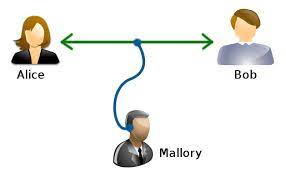
\includegraphics[scale=0.5]{Figs/bobalice.jpg}
    \caption{Bob e Alice}
    \label{fig:bobalice}
\end{figure}
Exemplificando, tem-se as seguintes etapas na utilização de uma cifra:
\begin{description}
    \item[Utilização de uma cifra de chaves simétricas] {\ }
    \begin{enumerate}
        \item Alice e Bob escolhem (secretamente) um par de chaves;
        \item Bob decide enviar uma mensagem, $m \in \mathcal{M}$, a Alice. Calcula $c=E_e(m)$ e envia o texto resultante;
        \item Ao receber a mensagem a Alice calcula $D_d(c)=m$ recuperando deste modo a mensagem original.
    \end{enumerate}
    \item[Utilização de uma cifra de chaves assimétricas] {\ }
    \begin{enumerate}
        \item O Bob escolhe um par de chaves: torna pública a chave de encriptação $e$, mantém secreta a chave de desencriptação $d$.
        \item A alice decide enviar uma mensagem, $m \in \mathcal{M}$, ao Bob. Obtém a chave pública do Bob $e$ e calcula $c=E_e(m)$. Depois envia o texto resultante.
        \item Ao receber a mensagem o Bob calcula $D_d(c)=m$ recuperando deste modo a mensagem original.
    \end{enumerate}
\end{description}

Assim, Bob e Alice conseguem comunicar secretamente, sem conceder ao Mallory acesso ao conteúdo da conversa.

Naturalmente todo o código têm duas etapas: uma para codificar a mensagem e outra para decodificar a mensagem. Mas para decifrar uma mensagem, isto é, ler um mensagem codificada sem ser o verdadeiro destinatário dela é preciso ``quebrar'' o código. Portanto é necessário introduzir a seguinte definição:

\begin{definicao}[Criptoanálise] É o estudo dos procedimentos necessários para tentar comprometer as técnicas criptográficas, e mais genericamente, os serviços de segurança da informação.
\end{definicao}

\begin{definicao}[Cifra (parcialmente) Quebrada] É o ataque sistemático a uma cifra com a finalidade principal de obter texto claro a partir de texto cifrado. Em caso de sucesso, diz-se que a cifra for parcialmente quebrada.
\end{definicao}

\begin{definicao}[Cifra (formalmente) Quebrada] Tem por objetivo obter a chave privada de uma entidade, nesse caso a cifra é completamente e formalmente quebrada.
\end{definicao}

Relativamente as classes de ataques aos esquemas de encriptação, tem-se as seguintes definições:

\begin{definicao}[Ataque Passivo] É um ataque em que o adversário apenas monitoriza o canal de comunicação. Um atacante passivo apenas ameaça a confidencialidade da informação.
\end{definicao}

\begin{definicao}
[Ataque Ativo] É um ataque em que o adversário tenta apagar, acrescentar, ou de alguma forma modificar a informação. Um atacante ativo ameaça a integridade da informação assim como a sua confidencialidade.
\end{definicao}

Em relação ao tipo de ataque, tem-se as seguintes definições:

\begin{definicao}[Ataque de texto cifrado] neste tipo de ataque o criptoanalista tenta deduzir a chave de decifração ou o texto claro por observação unicamente do texto cifrado. Uma cifra que seja vulnerável a este tipo de ataque considera-se completamente inseguro.
\end{definicao}

\begin{definicao}[Ataque de texto claro conhecido] É um ataque aonde o criptoánlista consegue obter um excerto de um texto claro com base num seu corresponde teste cifrado.
\end{definicao}

\begin{definicao} [Ataque de texto claro escolhido]É um ataque aonde o adversário escolhe o texto em claro obtendo de seguida o corresponde texto cifrado. Toda a informação daí deduzida é posteriormente usada em outros textos cifrados.
\end{definicao}

\begin{definicao} [Ataque de de força bruta] É um ataque por procura exaustiva no espaço das chaves. Uma cifra sujeita a este tipo de ataque é designado por cifra fraca.
\end{definicao}


Por exemplo, suponhamos que o Mallory, extremamente perspicaz, conseguiu encontrar uma forma de comprometer os métodos de encriptação e desencriptação utilizados pelo Bob e a Alice. Primeiramente, efetuou a monitorização das conversas trocadas pelo Bob e Alice tendo conseguido chegar ao texto cifrado a partir de um certo texto original que conseguiu reunir antes do Bob enviar para a Alice. 
Apercebendo-se do quanto o conteúdo da informação era preciosa, Mallory quis impedir Alice de ter acesso ao resto do informação.
Para isso encontrou a chave certa testando todas as chaves disponíveis. E com isso conseguiu,facilmente, decifrar o conteúdo dos textos cifrados do Bob e passou a enviar falsas correspondências, em nome do Bob, a alice.
\begin{figure}[h]
    \centering
    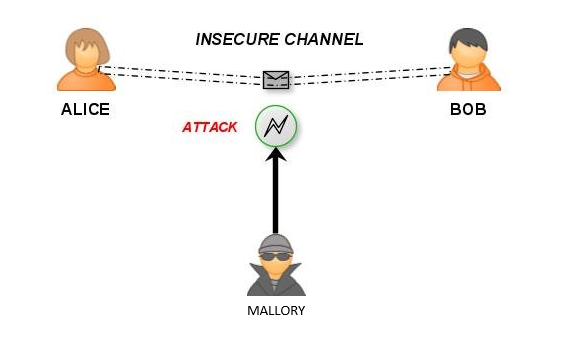
\includegraphics[scale=0.5]{Figs/mallory.PNG}
    \caption{Bob, Alice e Mallory}
    \label{fig:bobalice}
\end{figure}

Observação: Num sistema de chave pública é preciso saber a chave pública do destinatário de modo a encriptar uma mensagem a ele destinada. Apenas o destinatário é capaz de decifrar a mensagem.

Nota: Cada entidade tem um par (chave pública, chave privada). De forma a evitar ataques as chaves públicas disponibilizadas pelas entidades, tais como, a substituição da chave pública (este tipo de ataque é designado por personificação) foi criado um repositório de chaves que é capaz de garantir a manutenção das chaves~\cite{Quaresma2009a}.


\chapter{Criptografia Clássica}

Designa-se usualmente por \emph{criptografia clássica} as cifras  pré-computacionais, desenvolvidas e utilizadas tendo por base processos mecânicos ou manuais. O mais simples deste tipo de criptografia consiste em trocar uma letra pela seguinte. Um código similar foi usado por Júlio César, cuja a chave era estabelecida pelo deslocamento, de três posições, nas letras do alfabeto~\cite{Coutinho2005}.

\begin{definicao}[Cifra Deslocamento]
 Seja $\mathcal{M}=\mathcal{C}=\mathbb{Z}_{26}^*$, $\mathcal{K}=\mathbb{Z}_{26}$. 7
 Para $0 \leq K \leq \mid\mathbb{Z}_{26}\mid$=26, define-se:
$$e_k(x)=(x+K) \; mod \; 26$$ e $$d_k(y)=(y - K) \; mod \; 26$$ para todo o $x,y \in \mathbb{Z}_{26}$
\end{definicao}

\emph{Nota:} para $\mathbb{Z}_{n}$ tem-se $n=26$ uma vez que o alfabeto adotado tem 26 caracteres.

\begin{teorema}[Cifra Deslocamento Simples] As funções $e_k$ e $d_k$ constituem uma cifra.
\end{teorema}
\begin{demonstracao}
    \begin{align*}
    d_k(e_k(x)&=d_k(x+k)=\\
              &=(x+k)-k=\\
              &=x\;mod\;26
\end{align*}

Então, por definição,a cifra de deslocamento é uma cifra.
\end{demonstracao}


\begin{definicao}[Cifra Deslocamento Linear]
    Seja $\mathcal{M}=\mathcal{C}=\mathbb{Z}_{26}^*$, e seja:
$K=\{(a,b) \in \mathbb{Z}\times \mathbb{Z} : mdc(a,26)=1\}$.

Para $K=(a,b) \in \mathcal{K}$, define-se:
$$ e_k(x)=(ax + b)\;mod\;26$$
e
$$ d_k(y)=a^{-1}(y - b)\;mod\;26$$
para todo o $x,y \in \mathbb{Z}_{26}$
\end{definicao}

\begin{teorema}[Cifra deslocamento linear] As funções $e_k$ e $d_k$ constituem uma cifra.
\end{teorema}
\begin{demonstracao}
    \begin{eqnarray*}
    d_k(e_k(x)) & = & d_k(ax +b)\\
                & = & a^{-1}(ax+b -b)\quad\text{\;por definição $a$ é invertível em $\mathbb{Z}_{26}$}\\
                & = & a^{-1}ax\\
                & = & x
    \end{eqnarray*} 
Por definição, verifica-se que o resultado apresentado anteriormente é verdadeiro.
\end{demonstracao}


Relativamente à criptoanálise, as cifras clássicas são cifras muito fracas ou completamente inseguras pelo que estão suscetíveis a ataques por procura exaustiva. Também é possível quebrar esta cifra por ataques baseada na frequência relativa das letras, diagramas,trigramas, letras iniciais e finais das palavras.

Por exemplo, se todas as todas as ocorrências da letra $a$ são substituídas pela letra $x$, uma mensagem cifrada contendo muitas instâncias da letra $x$, iria sugerir ao criptoanalista, que a letra $x$ representa a letra $a$.

De facto, para uma dada linguagem verifica-se que cada letra aparece de acordo com uma frequência própria. No caso da língua portuguesa tem-se a seguinte tabela de frequência:~\cite{Quaresma2009a}:

\begin{table}[h]
\centering
\begin{tabular}{>{\columncolor{gray!20}}cccccccccc}
a & 12,71\% & \cellcolor{gray!20}b & 0.81\% & \cellcolor{gray!20}c & 4,16\% & \cellcolor{gray!20}d  & 5,52\% & \cellcolor{gray!20}e & 11,99\% \\
f & 1,43\% & \cellcolor{gray!20}g & 1,32\% & \cellcolor{gray!20}h & 0,74\% & \cellcolor{gray!20}i  & 7,18\% & \cellcolor{gray!20}j & 0,21\% \\
k & 0,00\% & \cellcolor{gray!20}l & 3,23\% & \cellcolor{gray!20}m & 4,48\% & \cellcolor{gray!20}n  & 5,24\% & \cellcolor{gray!20}o & 11,32\% \\
p & 3,07\% & \cellcolor{gray!20}q & 1,41\% & \cellcolor{gray!20}r & 6,47\% & \cellcolor{gray!20}s  & 7,99\% & \cellcolor{gray!20}t & 5,31\% \\
u & 3,44\%  & \cellcolor{gray!20}v & 1,36\% & \cellcolor{gray!20}w & 0.02\% & \cellcolor{gray!20}x  & 0,28\% & \cellcolor{gray!20}y & 0,02\% \\
z & 0,37\% & & & & & &  & & \\
\end{tabular}
\end{table}

Com estes dados, agrupa-se estes valores em grupos, das letras com maior frequência para as menos frequentes:

\begin{table}[h]
\centering
\begin{tabular}{>{\columncolor{gray!20}}ccccc}
Primeiro grupo  & \cellcolor{gray!20}Segundo grupo & \cellcolor{gray!20}Terceiro grupo & \cellcolor{gray!20}Quarto grupo  & \cellcolor{gray!20}Quinto grupo\\
a,e,o &s,r,i & n,d,m,u,t,c &  l,p,v,g,h,q,b,f  & z,j,x,k,w,y\\
\end{tabular}
\end{table}

Notar que este processo reduz o número de tentativas e erro a realizar antes de se conseguir quebrar o código tornando-o mais eficiente.

Logo para quebrar a cifra utilizada para obter o texto encriptado ``a fkdyh whp gh vhu pdqwlgd', sabendo que foi utilizado um sistema de cifração de deslocamento simples, precisamos de calcular as frequências relativas para o texto cifrado,tem-se:


\begin{table}[h]
\centering
\begin{tabular}{>{\columncolor{gray!20}}cccccccccc}
d & 17,9\% & \cellcolor{gray!20}f & 7,1\% & \cellcolor{gray!20}g & 7,1\% & \cellcolor{gray!20}h & 21,4\% \\
k & 3,6\% & \cellcolor{gray!20}l & 3,6\% & \cellcolor{gray!20}p & 7,1\% & \cellcolor{gray!20}q & 3,6\% \\
u & 7,1\% & \cellcolor{gray!20}v & 7,1\% & \cellcolor{gray!20}w & 10,7\% & \cellcolor{gray!20}y & 3,6\% \\
\end{tabular}
\end{table}
Por análise das frequências relativas e consultado o primeiro grupo, onde as letras tem maior frequência relativa, uma vez que ``d'', com $17,9\%$, e o ``h'', com $21,4\%$ então podemos fazer ``d'' corresponder a ``a'', por exemplo. Neste caso, a nossa chave é 3.

Assim, obtemos o texto claro ``a chave tem de ser mantida secreta''. Logo a cifra foi quebrada.~\cite{Quaresma2009a}

Com recurso do computador podemos facilmente realizar todo o processo anterior rapidamente pelo que este tipo de cifra é muito fraca.
 \chapter{Criptografia RSA}
\label{sec:criptografiaRSA}

Metódo de criptografia de chave pública criado em 1978 por R.C. \textbf{R}ivest, A. \textbf{S}hamir e L.\textbf{A}dlemar(RSA), que na época trabalhavam no massachusetts Institute of Tecnology(MIT). Presentemente, é o código de chave pública mais utilizado em aplicações comerciais~\cite{Coutinho2005}.

Para implementar a criptografia RSA vamos precisar de:
\begin{itemize}
    \item escolher dois  números primos de grande dimensão,\footnote{Size considerations for public and private keys, \url{https://www.ibm.com/docs/en/zos/2.3.0?topic=certificates-size-considerations-public-private-keys}} $p$ e $q$;
    \item conhecer $n=pq$ para codificar a mensagem;
    \item saber $p$ e $q$ para decodificar a mensagem;
\end{itemize}

A segurança do metódo advêm da dificuldade que é fatorizar números primos, uma vez que para descobrir a chave de encriptação é preciso fatorizar n de forma a encontra $p$ e $q$.

Seja $\mathcal{C}_p=(e,n)$ Chave Pública, onde $1 < e <\phi(n)$. Tem-se, pela função de Euler e \emph{teorema~\ref{teo:teoremaA}}, $mdc(e,\phi(n))=mdc(e,(p-1)(q-1))=1$

Seja $\mathcal{C}_s=(d,n)$  Chave Privada, onde $d$ é o inverso multiplicativo de $e$(Proposição 2), módulo $\phi(n)$.

O algoritmo de encriptação, $\mathcal{A}_{C_p} \;: \; M \; \to \mathcal{A}_{C_p}(M)$, é:
$$C=M^e(mod \; n)$$
O algoritmo de desencriptação, $\mathcal{A}_{C_s} \;: \; C \; \to \mathcal{A}_{C_s}(C)=M$, é:
$$M=C^d(mod \; n)$$

Para que o algoritmo RSA possa ser considerado uma cifra o procedimento tem de ser invertível, isto é,
$$A_{C_s}(A_{C_P}(M))=A_{C_P}(A_{C_s}(M))=M^{ed}(mod \; n)= M$$

\section{Teorema RSA}

Para provar este resultado vamos precisar da congruência $\mod m$ e da consequência que daí se tira que se $a \equiv b ( mod \; n)$ então $a=b +kn $, para um dado $k \in \mathbb{Z}$.

Para o desenvolvimento da demonstração são necessários alguns resultados auxiliares, nomeadamente, congruência $\mod m$, \emph{pequeno teorema de Fermat} e \emph{teorema chinês dos restos}.

\begin{teorema}[Cifra RSA]
Sendo $(e,n)$ e $(d,n)$ as chaves públicas e privada respetivamente do sistema de Criptografia RSA verifica-se então que:
$$(m^e)^d(mod \; n)=m$$
para qualquer inteiro $m$, com $0 \le m < n$.
\end{teorema}

\begin{demonstracao}
Da definição de $e$ e $d$ tira-se que $ed \equiv 1 (mod \; \phi(n))$ existe então um $k \in \mathbb{Z}$ tal que $ed= 1+ k\phi(n)$, ou seja:
$$ed=1+k(p-1)(q-1), \; K \in \mathbb{Z}$$
donde
$$(m^e)^d=m^{ed}=m^{1+k(p-1)(q-1)}=m(m^{(p-1)(q-1)})^k$$
segue-se que
$$(m^e)^d \equiv m(m^{(p-1)})^{(q-1)k} \equiv m(mod p)$$
Se $p$ não é um divisor de $m$ esta congruência é uma consequência do \emph{pequeno teorema  de fermat}. Caso contrário a asserção é trivial dado que ambos os membros da equação são congruentes com $0 \; mod \; p$.

De forma análoga ter-se-ia que:
$$(m^e)^d \equiv m\;(mod \; q)$$

Dado que $p$ e $q$ são números primos distintos pode-se aplicar o teorema chinês dos restos e dado que se assume que $0 \le m < n$, obtêm-se~\cite{Quaresma2009a}:
$$(m^e)^d \equiv m\;(mod \; pq) \equiv(mod \; n)=m$$
\end{demonstracao}

\subsubsection{Porque o RSA é seguro?}
\label{sec:porqueeRSAeseguro}

Seja $p$ e $q$ os parâmetros que estamos a utilizar. Sendo o RSA um método de chaves públicas então a chave de codificação corresponde a chave pública do sistema, ou seja, o par $(n,e)$ é acessível a qualquer utilizador. Logo a segurança do RSA provém da dificuldade do cálculo de $d$ sabendo $n$ e $e$.

Efetivamente, apenas sabemos calcular $d$ por aplicação do algoritmo de Euclides a $\phi(n)$ e $e$. Por outro lado, apenas consegue-se calcular $\phi(n)$ se formos capazes de fatorizar $n$ de forma a obter $p$ e $q$, isto é, apenas é possível quebrar o código se conseguirmos fatorizar $n$.

Além disso, é impossível alguém criar uma forma de descobrir $d$ sem ter que fatorizar.
De facto, a partir de $n=pq$ e $\phi(n)=(p-1)(q-1)$ conhecidos tem-se
$$\phi(n)=(p-1)(q-1)=pq-(p+q)+1=n-(p+q)+1$$
tal que $p+q=n-\phi(n)+1$ é conhecido. Mas
$$(p+q)^2-4n0(p^2+q^2+2pq)-4pq=(p-q)^2$$
Logo
$$p-q=\sqrt{(p+q)^2-4n}$$
Assim sabendo $p+q$ e $p-q$ calcula-se facilmente $p$ e $q$~\cite{Coutinho2005}.

%\textbf{Criptoanálise}
%\addcontentsline{toc}{section}{Criptoanálise}
\section{Criptoanálise}
\label{sec:criptoanalise}

Ao longo dos anos, vários métodos de criptoanálise têm sido desenvolvidos para tentar encontrar vulnerabilidades no algoritmo RSA e em outros sistemas criptográficos. Estes incluem ataques de fatoração de inteiros, ataques de timing, entre outros, cada um com vista a encontrar falhas na segurança para comprometer a proteção dos dados~\cite{Quaresma2009a,Coutinho2005}.

A contínua evolução da criptoanálise e a descoberta de nova formas de ataque salientam a importância de manter algoritmos como o RSA em constante revisão e atualização, de modo a garantir assim a segurança dos dados em um ambiente digital em constante mudança e cada vez mais propenso a ameaças cibernéticas.

Em seguida são apresentados alguns dos métodos de criptoanálise,  que em casos específicos, conseguem quebrar a cifra RSA.

\begin{comment}
\textbf{Expoente de encriptação}

De maneira a aumentar a eficiência da encriptação é importante selecionar um expoente d encriptação $e$ pequeno
$$c=m^e(mod \; n)$$
Mas $e$ não poder ser muito pequeno. Com efeito para $e=3$ suponhamos que estamos a enviar a mensagem $m$ para três diferentes entidades com módulos públicos de $n_1, \;n_2 \; e n_3$, vai se enviar $c_i=m^3 mod\;n_i$ para $1\le\le 3$.\\
Consideremos que $n_1,n_2 e n_3$ são primos dois a dois, é possível usar os textos encriptados para descobrir a solução $x$, onde $0 \le x \le n_1n_2n_3$, das três congruências anteriores vamos obter 
\begin{equation}
\left\{ \begin{aligned} 
  x &\equiv c_1 (mod \;n_1)\\
  x &\equiv c_2 (mod \;n_2)\\
  x &\equiv c_3 (mod\;n_3)\\
\end{aligned} \right.
\end{equation}
Uma vez que $n^3 < n_1n_2n_3$, pelo Teorema Chinês dos Restos, tem-se que $x=m^3$. Logo fazendo a raiz cúbica de x consegue-se recuperar o texto original.[4]
\end{comment}

\subsection{Método de Fermat}
\label{sec:metodoFermat}

Proposto Pierre Fermat para encontrar dois inteiros a e b que permitam representar o número natural n como diferença de dois quadrados:
$$n=a^2\;-\;b^2 \leftrightarrow n=(a\;-\;b)(a\;+\;b)$$

\begin{teorema}
qualquer inteiro $n$ ímpar maior que 1 pode ser escrito como a diferença de dois quadrados.
\end{teorema} 

\begin{demonstracao}
Seja $n=pq$, com $q\le p$(no caso de $n$ ser primo considera-se $n=n \times 1$).
Por hipótese $n$ é ímpar, então $p$ e $q$ também o são, logo:$\frac{p+q}{2}$ e $\frac{p-q}{2}$ são inteiros, ma então temos:
\begin{align*}
    \left(\frac{p+q}{2}\right)^2-\left(\frac{p-q}{2}\right)^2&=\frac{p^2+2pq+q^2}{4}-\frac{p^2-2pq+q^2}{4}\\
    &=\frac{p^2+2pq+q^2-p^2+2pq-q^2}{4}\\
    &=\frac{4pq}{4}\\
    &=pq\\
    &=n
\end{align*}
\end{demonstracao}

Para determinar os inteiros $a$ e $b$ de forma que $n=a^2 - b^2$, o processo pode ser conduzido da seguinte maneira:
\begin{itemize}
    \item Dado um inteiro $n$ ímpar começamos por $a=\lfloor \sqrt{n} \rfloor +1$
    \item Se $b=\sqrt{a^2-n}$ é um inteiro, obtém-se o pretendido
    \item Caso contrário, incrementamos a de uma unidade até que b seja um inteiro;
\end{itemize}

Por exemplo, para $n=2027651281$temos 

$a=\lfloor \sqrt{n} \rfloor +1=45030$

Para b obteve-se a seguinte tabela de tentativas~\cite{Quaresma2009a}:

\begin{table}[h]
\centering
\begin{tabular}{>{\columncolor{gray!20}}cccc}
a & b & \cellcolor{gray!20}a & b\\
1º45030 & $\sqrt{45030^2-2027651281^2}=222,75$ & \cellcolor{gray!20}7º45036 & $\sqrt{45036^2-2027651281}=768,12$\\
2º45031 & $\sqrt{45031^2-2027651281^2}=373,73$  & \cellcolor{gray!20}8º45037 & $\sqrt{45037^2-2027651281^2}=824,67$ \\
3º45032 & $\sqrt{45032^2-2027651281}=479,31$ & \cellcolor{gray!20}9º45038 & $\sqrt{45038^2-2027651281}=877,58$\\
4º45033 & $\sqrt{45033^2-2027651281}=565,51$ & \cellcolor{gray!20}10º45049 & $\sqrt{45039^2-2027651281}=927,49$\\
5º45034 & $\sqrt{45034^2-2027651281}=640,21$ & \cellcolor{gray!20}45040 & $\sqrt{45040^2-2027651281}=974,84$\\
6º45035 & $\sqrt{45035^2-2027651281}=707,06$ & \cellcolor{gray!20}12º45041 & $\sqrt{45041^2-2027651281}=1020$\\
\end{tabular}
\end{table}


De 
\begin{equation}
\begin{cases}
    \frac{p+q}{2}=46041\\
    \frac{p-q}{2} = 1020
\end{cases}
\end{equation}

obtém-se $p=47061$ e $q=45021$

Assim $n=45041^2-1020^2$, $n=46061\times44021$.
Relativamente ao algoritmo de fermat prova-se que,quanto maior for a diferença entre $p$ e $q$, maior é o número de tentativas que vão ser precisas obter um primeiro valor inteiro para a raiz~\cite{Quaresma2009a}.

\subsection{Método das Divisões}

Neste método, a abordagem consiste em empregar a técnica da fatoração por tentativa, que requer a divisão iterativa por todos os números primos até chegar ao valor de $\lfloor \sqrt{n} \rfloor$ ou até que a solução seja identificada~\cite{Quaresma2009a}.

Para isso precisamos de gerar uma lista de números primos até ao limite pretendido. Presentemente, ainda não é conhecida nenhuma formula para gerar números primos. Assim, é necessário adotar um procedimento que apresente a enumeração exaustiva de todos os números primos até o limite especificado, tal como o algoritmo do Crivo de Eratóstenes.

\subsection{Crivo de Aristóteles}

O método do Crivo de Eratóstenes, criado pelo matemático grego Eratóstenes, representa um algoritmo prático e direto para determinar números primos até um certo limite. 

Para exemplificar, vamos listar os números primos de 1 a 30.

\begin{itemize}
    \item Primeiramente, precisamos determinar $\lfloor \sqrt{30} \rfloor$, o número limite a ser verificado;
    \item gerar uma lista de inteiros de 2 a 30;
    \item obter o primeiro número da lista, neste caso é o 2;
    \item eliminar todos os números da lista, excepto o 2;
    \item O número sucessor na lista após o primo anterior também é primo. 
\end{itemize}

Obviamente, se repetirmos esse raciocínio até ao final da lista anteriormente gerada, os elementos que não forem eliminados pelas sucessivas aplicações do crivos são números primos de 1 a 30.

Contudo a utilização deste algoritmo adiciona um elevado peso tanto em termos de tempo como de espaço uma vez que é preciso gerar o lista de inteiros de 2 a $n$ e estar a aplicar constantemente o crivo a lista~\cite{Quaresma2009a}.

Alternativamente, existem outros métodos capazes de produzir uma sequência de números primos, assim como números que não são primos com ganhos temporal e espacial comparativamente ao crivo de Aristóteles. Mas são, obviamente, menos eficientes a sua utilização~\cite{Quaresma2009a}.

\subsection{Método de Euclides}


Este metódo ganha o seu nome da utilização do algoritmo de Euclides para o cálculo do máximo divisor comum de dois inteiros. Este algoritmo é muito eficiente e pode ajudar-nos a obter um dos fatores primos de n, de forma a obter o factor primo desejado. Basta multiplicar todos os números primos entre 2 e $\lfloor \sqrt{n} \rfloor$., calcular de seguida o m.d.c entre esse produto e $n$, de forma a obter o factor primo desejado.

Este método recebe seu nome da utilização do algoritmo de Euclides para calcular o máximo divisor comum de dois números inteiros. Este algoritmo é muito eficaz e pode auxiliar na obtenção de um dos fatores primos de n. É suficiente multiplicar todos os números primos no intervalo de 2 a  $\lfloor \sqrt{n} \rfloor$, em seguida, calcular o máximo divisor comum entre esse produto e n para obter o fator primo pretendido.

Com este procedimento, obviamente, ainda vamos continuar com o mesmo problema de elevado peso temporal e espacial em consequência  da exigência de criar um registo de todos os números primos até um limite específico.

Por outro lado, vamos ter um problema de representação computacional decorrente dos número obtidos do produto de números primos uma vez que rapidamente o resultado excede a capacidade de representação da maioria das linguagens de programação disponíveis.
Para evitar esse problema final,  subdividi-se a operação de multiplicação em múltiplas multiplicações menores.

Para tal, os passos seguintes são adotados:

\begin{itemize}[itemsep=0pt]
    \item Começa-se por definir os conjuntos auxiliares:

    $R={r_1,r_2,\dots,r_n}$, representando $r_i$ um limite inferior $(r_1=1,\;r_i<r_{i+1});$
    
    $S={s_1,s_2,\dots,s_n}$, representando $s_i$ um limite superior$(s_i<s{i+1},s_{m-1}<\lfloor \sqrt{n} \rfloor<s_m)$;
    \item Para cada par $r_i$ e $s_i$, multiplicam-se todos os números primos entre estes dois limites, $P_i=\prod_{r_i\leq p_i \leq s_i}p_i$;
    \item Para cada um dos $P_i$ calcula-se o $mdc(P-i,n)=a_i$;
    \item Se $a_i \neq 1 $, então $a_i$ é o factor primo de $n$ que se pretende obter~\cite{Quaresma2009a}.
\end{itemize}

Para exemplificar, seja $n=1223$. Tem-se $\lfloor \sqrt{1223} \rfloor =34$, e realizemos a adição de forma iterativa, agrupando de 10 em 10.

$$R=\{1,11,21,31\} \; \; S=\{10,20,30,40\}$$

 $P_1=\prod_{1\leq 10 \leq s_1}p_1=2\times 3 \times 5 \times 7=210,\;mdc(210,1223)=1$
 
$P_2=\prod_{11\leq p_2 \leq 20}p_2=11\times 13 \times 17 \times 19=46189,\;mdc(46189,1223)=1$

$P_3=\prod_{21\leq p_3 \leq 30}p_i=23\times 29=667,\;mdc(667,1223)=1$

$P_4=\prod_{31\leq p_3 \leq 30}p_i=31\times 37=1147,\;mdc(1147,1223)=31$

Como foi dito anteriormente, embora este método seja muito eficiente, mesmo considerando o problema inicial anteriormente descrito, vai  prontamente resultar em problemas de representação devido à capacidade limitada dos tipos de dados disponíveis na maioria das linguagens de programação~\cite{Quaresma2009a}.

\subsection{Estudo Comparativo dos Vários Métodos}
\label{sec:EstudoComparativoVariosMetodos}

Vimos que do ponto de vista teórico existem abordagens construtivas de decomposição em números primos que podem ser empregadas para alcançar o objetivo. Entretanto, é importante avaliar se existem ferramentas computacionais viáveis para realizar essa quebra de maneira eficiente e prática.

Para analisar isso, uma vez que a análise da complexidade dos algoritmos apresentados está além do âmbito deste texto, simplesmente vamos exibir os resultados de um estudo comparativo dos diferentes métodos com base em um conjunto de testes de execução.

Cada dado foi adquirido de testes executados em condições computacionais uniformes:sistema windowns 10 home,Intel(R) Core(TM) i3-7020U CPU 2.30GHz, RAM 4 GB.

\begin{table}[h]
\centering
\caption{Estudo comparativo dos métodos}
\label{tab:EstudoMetodo}
\begin{tabular}{>{\columncolor{gray!20}}ccccc}
n & \cellcolor{gray!20}Fatores & \cellcolor{gray!20}Divisão & \cellcolor{gray!20}Euclides & \cellcolor{gray!20}Fermat\\
$1457$ & $p=31$, $q=47$ & $0,000$s & $0s$&$0s$\\
13199 &$p=67$, $q=197$&$0,002s$ & $0.002s$& $0s$\\
$281161$ & $p=79$, $q=3559$  & $0.136$s& $0.145s$&$0s$\\
$701123$ & $p=3559$, $q=197$ &$0.521$s& $0.482s$&$0.003s$\\
$23420707$&$p=41017$, $q=571$ & $71.124s$ & $64.86s$&$0s$\\
$488754769$ & $p=110503$, $q=4423$  & $-$ & $-$&$0.005s$\\
$2027651281$ & $p=46061$, $q=41017$ & $-$ & $-$&$0s$\\
$103955963689$ & $p=47188363$, $q=2203$  & $-$& $-$&$1.75s$\\
$210528952589$ & $p=95564663$, $q=2203$  & $-$ & $-$&$3.635s$\\
$2746662891777043$ & $p=47188363$, $q=58206361$  & $-$ & $-$&$0.024s$\\
$4509540007616669$ & $p=47188363$, $q=95564663$  & $-$ & $-$&$0.299s$\\
\end{tabular}
\end{table}


Podemos afirmar que, com a escolha correta dos fatores primos, a cifra RSA permanece protegida. De facto:
\begin{itemize}
    \item[] Os métodos de Divisão e Euclides não apenas observam um aumento significativo no tempo de execução à medida que os fatores primos crescem de maneira substancial, mas também perdem a capacidade de resolver o problema a partir de valores relativamente pequenos de $n=p\times q$. Essas limitações surgem da necessidade de gerar números primos até $\lfloor \sqrt{n} \rfloor$ e, no caso do método de Euclides, da multiplicação de números de grande escala.
    \item[]O método de Fermat observa um aumento muito acentuado em seus tempos de execução com o crescimento da dimensão dos fatores primos; no entanto, uma análise mais detalhada revela que quando os fatores primos estão em proximidade, o método de Fermat demonstra ser altamente eficaz.
\end{itemize}

Podemos inferir que, para garantir a segurança da criptografia RSA, os fatores primos devem estar consideravelmente distantes um do outro, e o valor de "n" deve ser maior que 20 dígitos\cite{Quaresma2009a}.

Efetivamente, o tamanho de $n$ deve ser consideravelmente maior. Devido a algoritmos mais eficazes do que os previamente mencionados, a criptografia RSA foi violada utilizando valores de $n$ contendo 129, 155 e até mesmo 576 dígitos. Atualmente, a cifra RSA emprega valores de $n$ com 1024 dígitos ou mais\cite{Quaresma2009a}.

\subsection{O Crivo quadratico - Algoritmo de Fatorização}

Ao longo da história, os matemáticos têm se dedicado em descobrir abordagens mais eficientes e rápidas para decompor números compostos.
No início, essa tarefa envolvia a tentativa de divisão por primos cada vez maiores até que a fatorização fosse obtida. Mas, esse método trivial só foi aperfeiçoado quando Fermat introduziu a ideia de fatorar a diferença de dois quadrados.
Para aplicarmos o método de Fermat, primeiramente seja $n$ o número a ser fatorizado. Em seguida, procuramos o menor quadrado que seja maior que $n$ e verificamos se a diferença entre esse quadrado e $n$ é um quadrado perfeito. Se for, aplicamos o método de fatorização da diferença de dois quadrados para encontrar os fatores de $n$. Caso contrário, continuamos a procurar  o próximo quadrado e repetimos o procedimento.

Apesar de o método de Fermat ser significativa melhor que o método da  divisão por  tentativa, o método de Fermat ainda é insuficiente quando se trata de fatorar números muito grandes, como os utilizados por exemplo na criptografia RSA, que podem ter centenas de dígitos. Nesse contexto, abordagens mais eficazes tornam-se imprescindíveis.

Outros procedimentos foram desenvolvidas ao longo do tempo, como o Método da Curva Elíptica, descoberto por H. Lenstra em 1987, e métodos probabilísticos, como os métodos de $p-1$ e $\rho$(Rho de Pollard) proposto por John Pollard em 1974 e 1975, respetivamente. Contudo, os algoritmos mais rápidos ainda continuam a adotar o mesmo princípio básico apresentado por Fermat. Tais como Método da Fração Contínua, que permitiu fatorizar números até 50 dígitos sendo na época o limite era 20.  Em seguida, também  o Crivo Quadrático e o Crivo de Corpos de Números que por sua vez possibilitaram fatorizar números com mais de 150.  Esses três últimos provieram diretamente do método de Briallart e Morrison.

Este texto destaca sobretudo o Crivo Quadrático, um método amplamente adotado e eficaz para fatorar números compostos. A sua importância na criptoanálise do RSA reside no facto de que ele possibilita a identificação e análise de possíveis fragilidades nos números primos empregados para formar as chaves criptográficas. Ao fatorar os números compostos envolvidos no algoritmo RSA, o Crivo Quadrático desempenha um papel fundamental na avaliação da segurança do sistema e na identificação de possíveis vulnerabilidades.

\subsection{O Crivo quadrático - Método de Fatorização}

O Crivo Quadrático, ou simplesmente chamado de QS, foi concebido por Carl Pomerance em 1981, expandindo as ideias anteriores dos matemáticos Kraitchik e Dixon. O QS foi o algoritmo de fatorização mais rápido conhecido até a descoberta do Crivo de Corpos de Números em 1993. Ainda assim, o QS é mais eficiente, simples e rápido para números inteiros com menos de 100 dígitos decimais. Trata-se de um método de fatorização de aplicação ampla, o que significa que a sua velocidade de processamento é determinada exclusivamente pelo tamanho do número inteiro a ser fatorado, sem considerar qualquer estrutura ou características específicas.

\subsection{Como Funciona}

Seja $n$ o número inteiro positivo que se pretende fatorizar. Tem-se como objetivo encontrar $x$ e $y$ inteiros tais que $x^2 \equiv y^2\pmod{n}$, aonde $xy$ é primo com $n$ e $x \not\equiv y \pmod{n}$.

De facto, isso é equivalente a $(x-y)(x+y) \equiv 0 \pmod{n}$ pelo que  o $mdc(x-y,n)$ e $mdc(x+y,n)$ são fatores de n.

Seja $$F(x)=(x+\lfloor \sqrt x \rfloor)^2 -n $$

onde   $x_1,x_2,x_3,\ldots,x_k$ inteiros não negativos. Pretendemos encontrar subconjuntos $x_{i1},x_{i2},\dots,x_{1t}$ dos $x_i's$ tal que 
$$F(x_{i1})F(x_{i2})\ldots F(x_{it})\equiv (x_{i1},x_{i2},\dots,x_{1t})^2\pmod n$$ é da forma $y^2$, ou seja,
onde $F(x_{i1})F(x_{i2})\ldots F(x_{it})=y^2.$


Por exemplo para $n=11649$, tem-se $\sqrt{1649}=40,607881…$ pelo que iniciamos da seguinte forma 

\begin{center}
\justify
Para $x_1=41$, $41^2 - 1649 = 1681 - 1649=32$ (não é um quadrado perfeito). \\
Para $x_1=42$, $42^2 - 1649 = 1764 - 1649 = 115$ (não é um quadrado perfeito). \\
Para $x_1=43$,$43^2 - 1649= 1849 - 1649= 200$ (é um quadrado perfeito).
\end{center}

Tem-se 
$32 \times 200=6400=80^2$ pelo que $$(41\times43)^2 \equiv 80^2 \pmod {1649}$$

Notar que $41\times43=1763 \equiv114 \pmod {1649}$ e $114 \not\equiv \pmod 80\pmod {1649}$. Portanto, $mdc(114-80,1649)=17$ pelo que $1649=1797$.Além disso, o subconjunto é $\{x_1,x_3\}$.

Pretendemos expandir essa mesma ideia para números muito maiores. Para isso, é necessário encontrar subconjuntos de $x_i's$ nas condições da definição anterior.

Primeiramente, é importante notar que se algum $x^2 \equiv \pmod {n}$ tiver um fator primo grande, então outro ${x'}^2 \equiv \pmod {n}$  precisará ter esse mesmo fator primo grande para que possamos juntar este resíduo no nosso conjunto. Por exemplo, no caso anterior para  n=1649, encontramos o segundo resíduo como sendo 115, que tem o fator primo maior 23 relativamente aos restantes, pelo que descartou-se o resíduo 115 do  produto final. 

Portanto precisamos de ter um limite B para o maior primo que pode ser aceite para fatorizar os resíduos que iremos obter.

\subsection{Como calcular B?}

\begin{definicao}[B-suave] Um inteiro positivo diz-se B-suave se nenhum dos seus fatores primos for maior   que B.
\end{definicao}

Seja \( m \) um inteiro positivo \( B \)-suave. Então existem \( p_1, p_2, \dots, p_{\pi(B)} \) tais que \( m = \prod p_i^{e_i} \), onde \( p_1, p_2, \dots, p_n \) são primos até \( B \) e cada \( e_i \geq 0 \). Consideremos $v(m)=(e_1,e_2,\dots,e_{\pi(B)})$ o vetor dos expoentes.

Portanto pelo  exemplo acima, tem-se

$32=2^5$

$115=2^3\times5^2$

$115=5\times23$

Logo no seguimento do raciocínio aplicado no exemplo anterior pretende-se saber quais dos resíduos \(B\)-suave devemos juntar de forma que possamos obter quadrados perfeitos por congruência. Nesse sentido, uma vez que para cada v os seus elementos correspondem ao valor dos expoentes dos fatores primo de um certo resíduo então visa-se estudar a dependência linear no nosso conjunto dos vetores 
 do espaço vetorial $\mathbb{F}_2^{\pi(B)}$. Isto é, pretende-se que o sistema $$Qv=0$$
 seja possível, onde Q é a matriz formada pelos vetores $v \in \mathbb{F}_2^{\pi(B)} $

Sabemos que, pelo resultado da álgebra, o nosso conjunto de vetores vai ser linearmente dependentes se tivermos pelo menos $\pi(B)+1$ números \(B\)-suave.

Ao escolher um valor pequeno para \(B\), temos a vantagem de não precisar de muitos elementos \(B\)-suaves para encontrar um subconjunto que seja um quadrado. No entanto, se \(B\) for muito pequeno, a condição de ser \(B\)-suave torna-se tão excecional que podemos não encontrar nenhum número que a satisfaça. Assim, é crucial encontrar um equilíbrio entre esses dois aspetos: o valor de \(B\) deve ser suficientemente pequeno para não requerer uma grande quantidade de números 
\(B\)-suaves para obtermos sucesso, mas também suficientemente grande para que esses números \(B\)-suaves ocorram com uma frequência adequada.

Vamos estimar o valor de \(B\) pela seguinte definição:

\begin{definicao}Seja $u^{-u}$ a probabilidade de $x^2 \pmod n$ ser \(B\)-suave, onde $u=\frac{1}{2}lnn/lnB$.
\end{definicao}

Antes de estimar \(B\) precisamos também considerar o tempo necessário para verificar a B-suavidade de $x^2-n$ para algum x. Ora, utilizando o crivo de Eratóstenes sabe-se que o tempo médio gasto em operações aritmética por x é $lnlnB$.

Então, se a probabilidade de um valor de \( x \) resultar em um número \( B \)-suave é \( u^{-u} \), então podemos esperar que aproximadamente \( u^u \) valores de \( x \) sejam necessários para obter um \( x \) bem-sucedido. Logo, para obter \( k+1 \) \( x \) bem-sucedidos, são necessários \( (k+1)u^u \) valores de \( x \).


Seja 

$$T(B) = u^u(k+1)\ln(\ln(B)), \quad \text{onde} \quad u = \frac{\ln(n)}{2\ln(B)}$$

Precisamos de introduzir o seguinte teorema.

\begin{teorema} [Hadamard and de la Vallée Poussin] Para $x \sim \infty
$,
$$\pi(B)\approx \frac{x}{lnx}$$
\end{teorema}

Queremos encontrar \(B\) como função de \(B\) que minimize $T(B)$. Visto que \(K \approx \frac{1}{2\pi(B)}\) está na ordem de grandeza de \(\frac{B}{\ln B}\), temos que $lnT(B) \sim S(B)$, onde $S(B)=ulnu + lnB$.

\begin{equation}
\frac{dS}{dB} = \frac{-\ln{n}}{2B\ln^2{B}}(\ln{\ln{n}} - \ln{\ln{B}} - \ln{2} + 1) + \frac{1}{B}
\label{eq:derivada}
\end{equation}

Quando definimos \eqref{eq:derivada} a zero, determinamos que \( \ln B \) está no intervalo entre \( c_1\sqrt{\ln n} \) e \( c_2\frac{1}{2}\sqrt{\ln\ln n} \) pelo que $lnlnnB \sim \frac{1}{2}lnln n$. 

Além disso, também temos que

$$lnB \sim \frac{1}{2}\sqrt{lnnlnlnn}$$
$$u \sim \sqrt{lnn/lnlnn}$$
$$S(B) \sim \sqrt{lnnlnlnn}$$




\chapter{Conclusões}
\label{sec:Conclusoes}
Ao longo do trabalho constatou-se o procedimento eficaz e seguro para criptografar a informação desempenhada  pela sistema RSA.

De facto, verifica-se na secção~\ref{sec:CriptoanaliseRSA} que os métodos analisados não têm capacidade de ``quebrar'' o método RSA em chaves maiores que 20 dígitos. As chaves seguras utilizadas atualmente para o algoritmo RSA têm cerca de 2048 bits.\footnote{Ver página: \emph{Size considerations for public and private keys}, \url{https://www.ibm.com/docs/en/zos/2.3.0?topic=certificates-size-considerations-public-private-keys}}

No próximo semestre, iremos aprofundar o estudo da criptoanálise do método RSA, com foco especial no crivo quadrático."



%%% Local Variables:
%%% mode: latex
%%% TeX-master: "../thesis"
%%% End:

%\include{Chapter7/chapter7}



% ********************************** Back Matter *******************************
%% Backmatter should be commented out, if you are using appendices after References

%\backmatter

% ********************************** Bibliography ******************************
\begin{spacing}{0.9}

% To use the conventional natbib style referencing
% Bibliography style previews: http://nodonn.tipido.net/bibstyle.php
% Reference styles: http://sites.stat.psu.edu/~surajit/present/bib.htm

\bibliographystyle{apalike}
%\bibliographystyle{plainnat} % use this to have URLs listed in References
\cleardoublepage
\bibliography{References/references} % Path to your References.bib file


% If you would like to use BibLaTeX for your references, pass `custombib' as
% an option in the document class. The location of 'reference.bib' should be
% specified in the preamble.tex file in the custombib section.
% Comment out the lines related to natbib above and uncomment the following line.

%\printbibliography[heading=bibintoc, title={References}]


\end{spacing}

% ********************************** Appendices ********************************

%\begin{appendices} % Using appendices environment

%% ******************************* Thesis Appendix A ********************************
\chapter{More information $\int$}

\section*{Carl Friedrich Gauss}

Johann Carl Friedrich Gauss (30 April 1777 -- 23 February 1855) was a German mathematician who contributed significantly to many fields, including number theory, algebra, statistics, analysis, differential geometry, geodesy, geophysics, electrostatics, astronomy, matrix theory, and optics.

Sometimes referred to as the Princeps mathematicorum (Latin, ``the Prince of Mathematicians'' or ``the foremost of mathematicians'') and ``greatest mathematician since antiquity'', Gauss had a remarkable influence in many fields of mathematics and science and is ranked as one of history's most influential mathematicians.

Gauss was a child prodigy. There are many anecdotes about his precocity while a toddler, and he made his first ground-breaking mathematical discoveries while still a teenager. He completed Disquisitiones Arithmeticae, his magnum opus, in 1798 at the age of 21, though it was not published until 1801. This work was fundamental in consolidating number theory as a discipline and has shaped the field to the present day.

Gauss's intellectual abilities attracted the attention of the Duke of Brunswick, who sent him to the Collegium Carolinum (now Braunschweig University of Technology), which he attended from 1792 to 1795, and to the University of G\"{o}ttingen from 1795 to 1798. While at university, Gauss independently rediscovered several important theorems; his breakthrough occurred in 1796 when he showed that any regular polygon with a number of sides which is a Fermat prime (and, consequently, those polygons with any number of sides which is the product of distinct Fermat primes and a power of 2) can be constructed by compass and straightedge. This was a major discovery in an important field of mathematics; construction problems had occupied mathematicians since the days of the Ancient Greeks, and the discovery ultimately led Gauss to choose mathematics instead of philology as a career. Gauss was so pleased by this result that he requested that a regular heptadecagon be inscribed on his tombstone. The stonemason declined, stating that the difficult construction would essentially look like a circle.

The year 1796 was most productive for both Gauss and number theory. He discovered a construction of the heptadecagon on 30 March. He further advanced modular arithmetic, greatly simplifying manipulations in number theory. On 8 April he became the first to prove the quadratic reciprocity law. This remarkably general law allows mathematicians to determine the solvability of any quadratic equation in modular arithmetic. The prime number theorem, conjectured on 31 May, gives a good understanding of how the prime numbers are distributed among the integers.

\section*{Another section}

\subsection*{Subsection}

\subsubsection*{Subsubsection}
...


%\end{appendices}


% *************************************** General Index ********************************
\printthesisindex % If index is present


\end{document}

%%% Local Variables:
%%% mode: latex
%%% TeX-master: t
%%% End:
